A potência necessária para alimentar o circuito de excitação de um alternador é, em geral, cerca de 5\% da potência do próprio alternador, variando a tensão de alimentação entre 50 e 250 volts. A corrente de excitação pode ser fornecida por um dínamo. Esse tipo de dínamo pode ser fixado sobre uma saliência do suporte do alternador, se este é horizontal, conforme as figuras abaixo.  

\begin{figure}[ht!]
\center
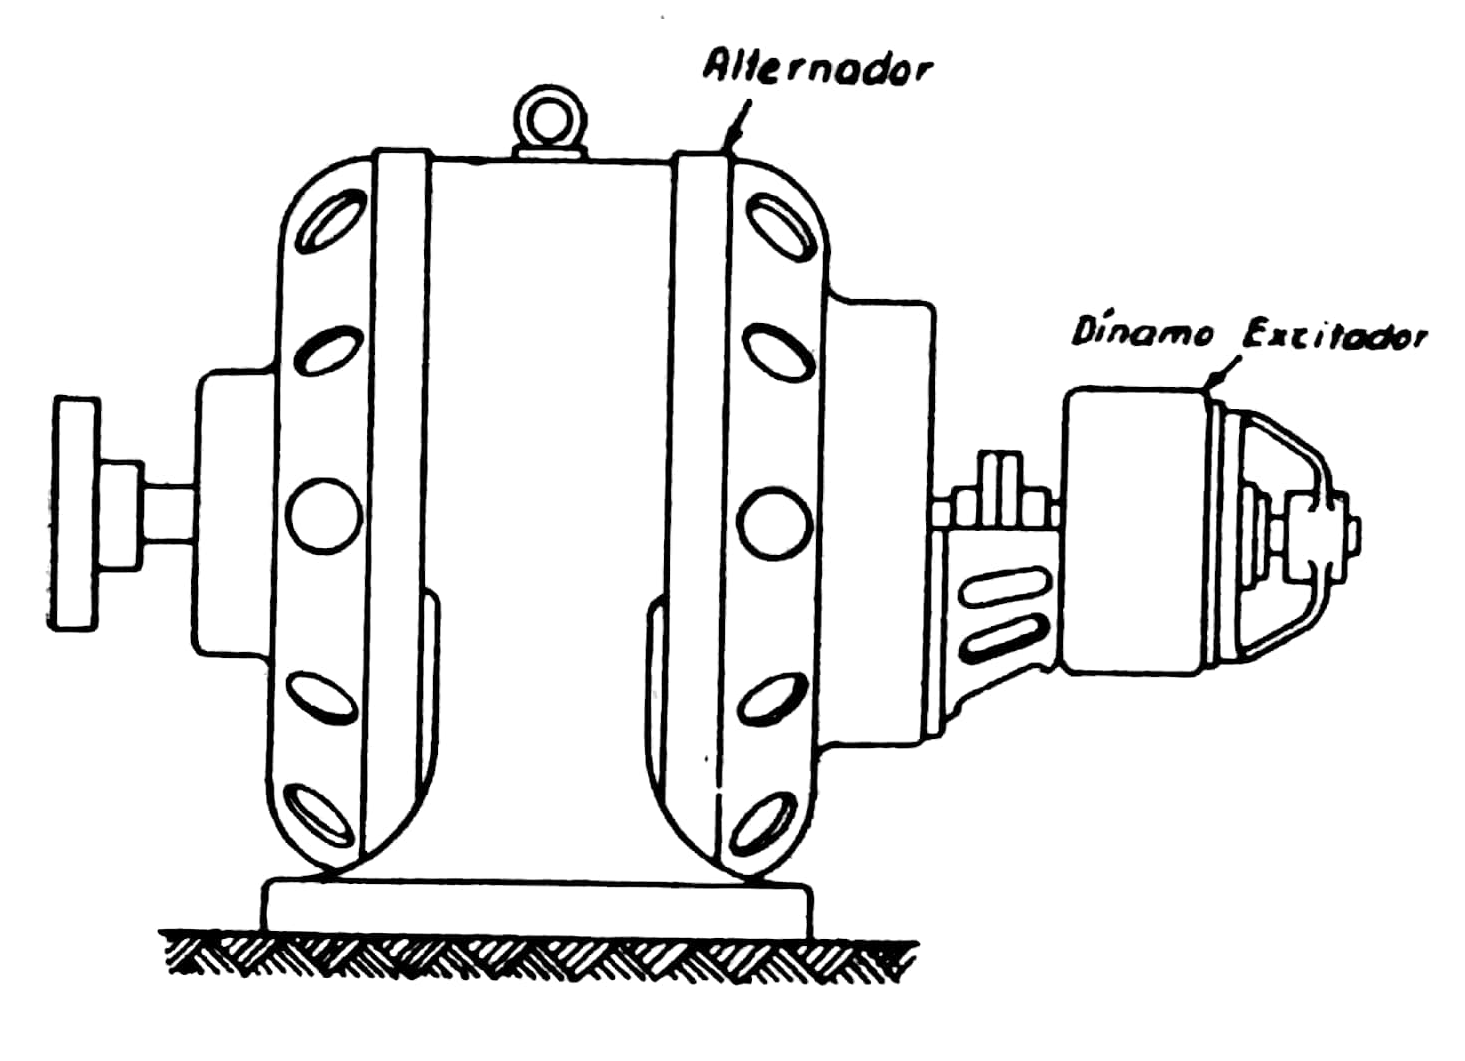
\includegraphics[scale=0.2]{imagens/17}
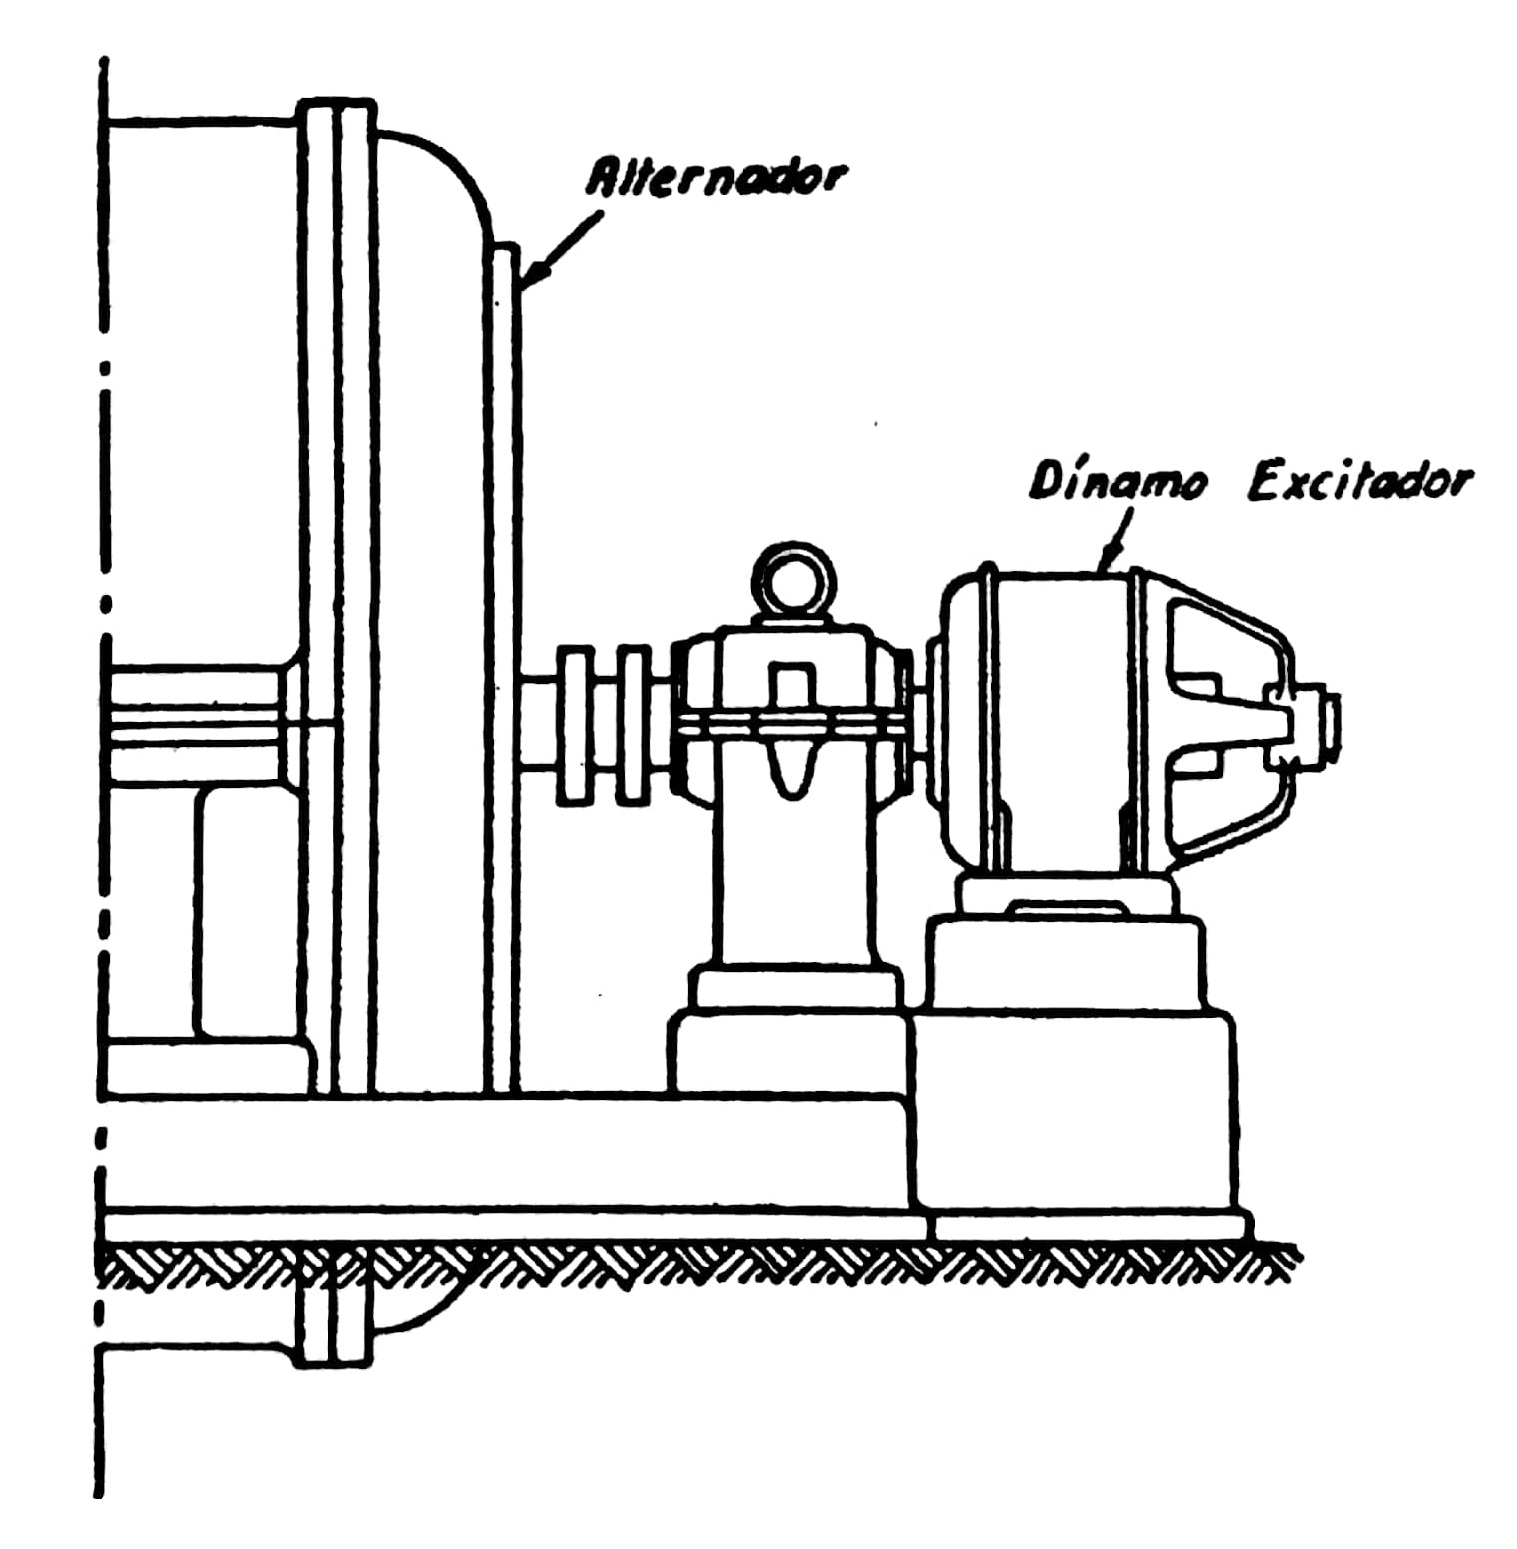
\includegraphics[scale=0.2]{imagens/18}
\caption{Alternadores Horizontais.}
\end{figure}

No caso de alternadores verticais, pode-se usar utilizar o suporte superior, conforme a figura a seguir.

\begin{figure}[ht!]
\center 
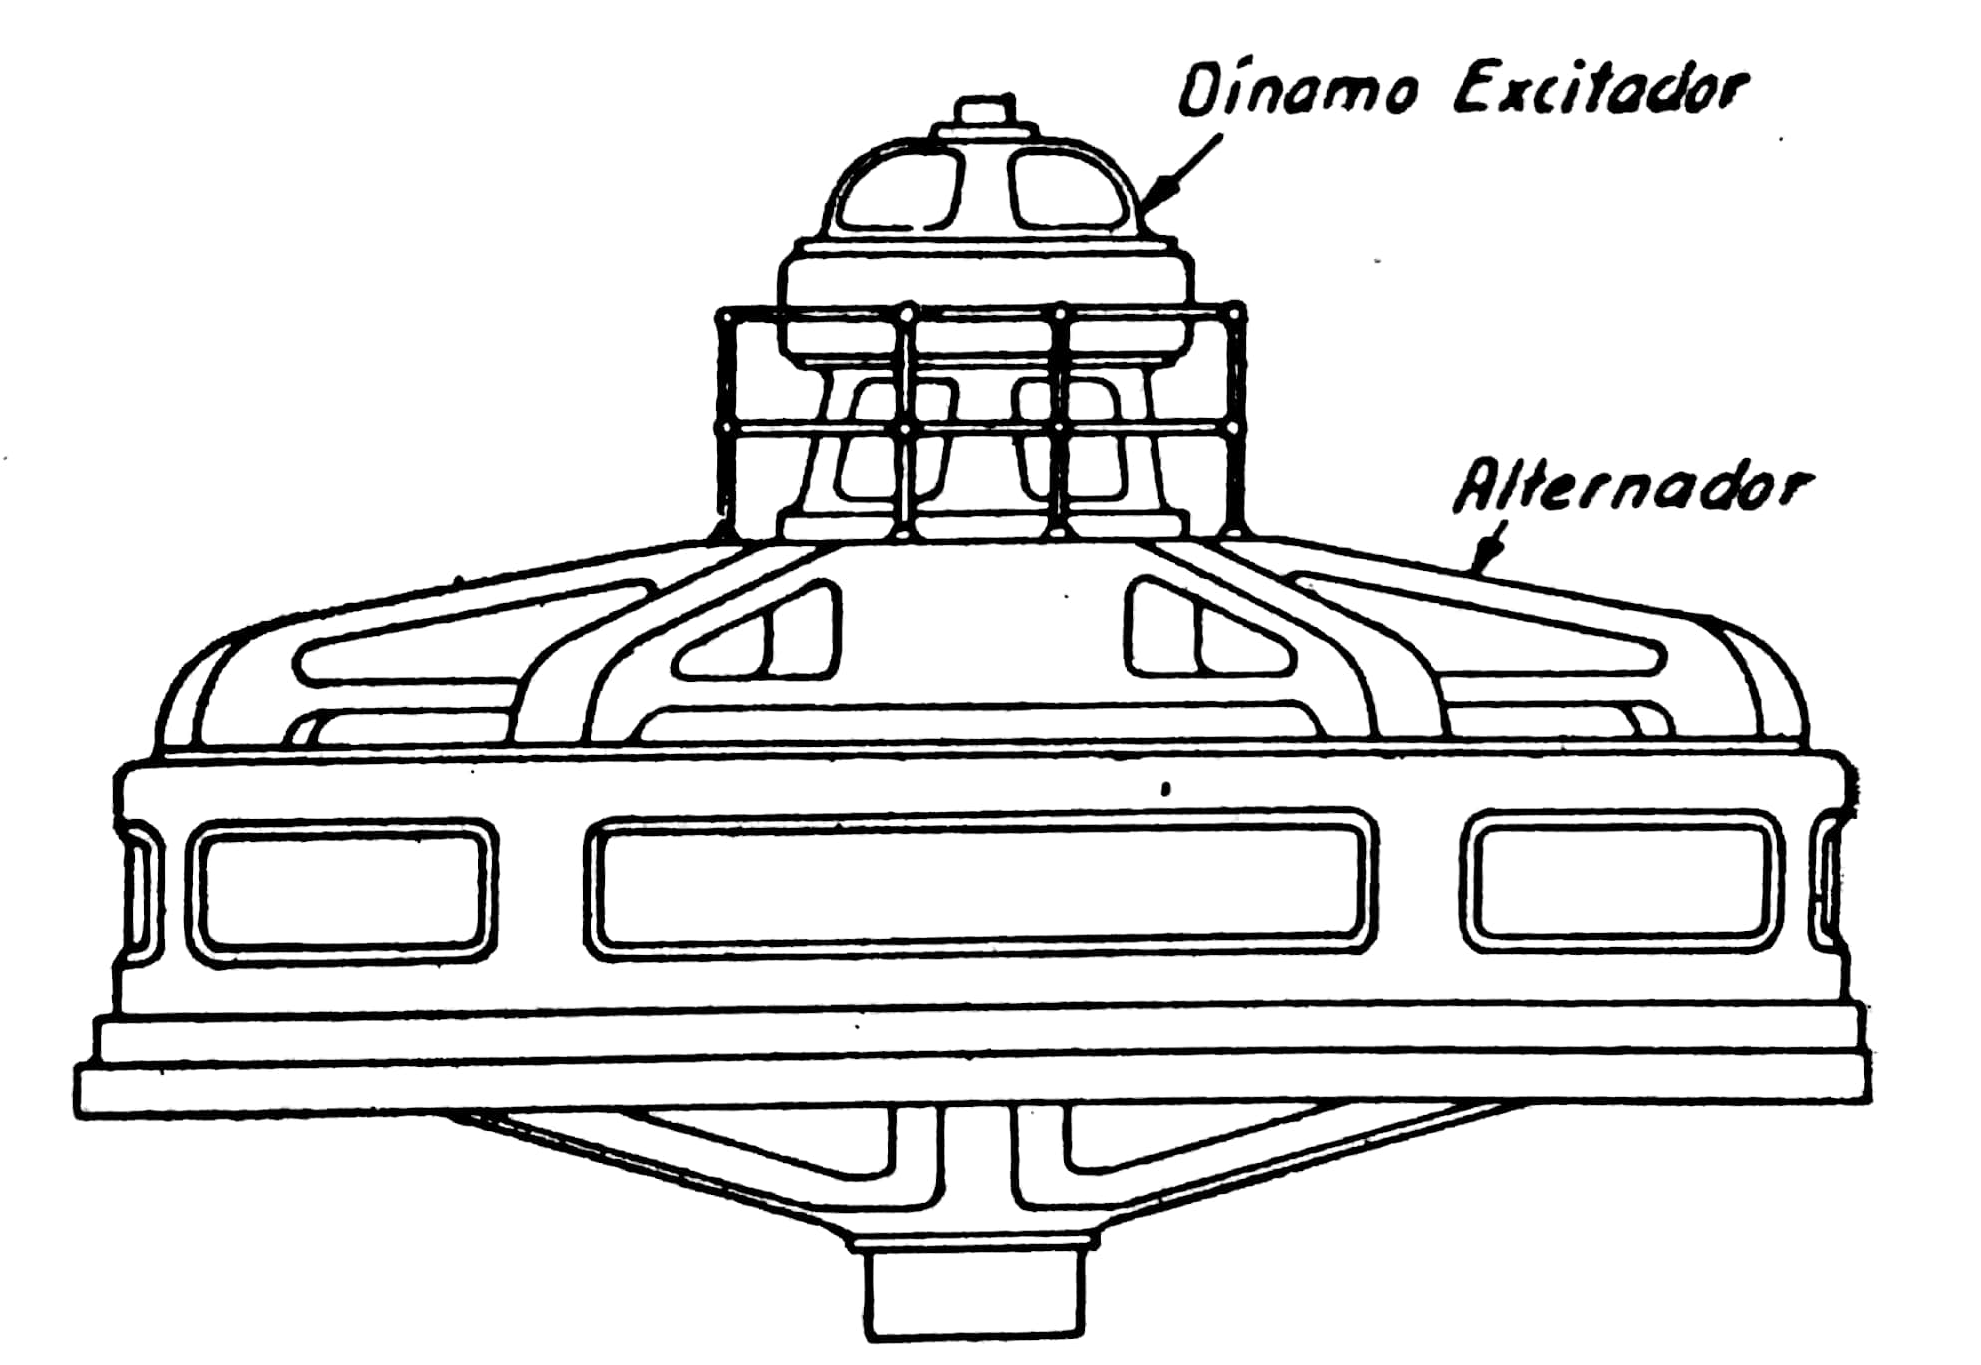
\includegraphics[scale=0.2]{imagens/16.png}
\caption{Alternador Vertical.}
\end{figure}
\newpage

O esquema elétrico relativo a este tipo de de excitação está representado na figura 21.

\begin{figure}[ht!]
\center 
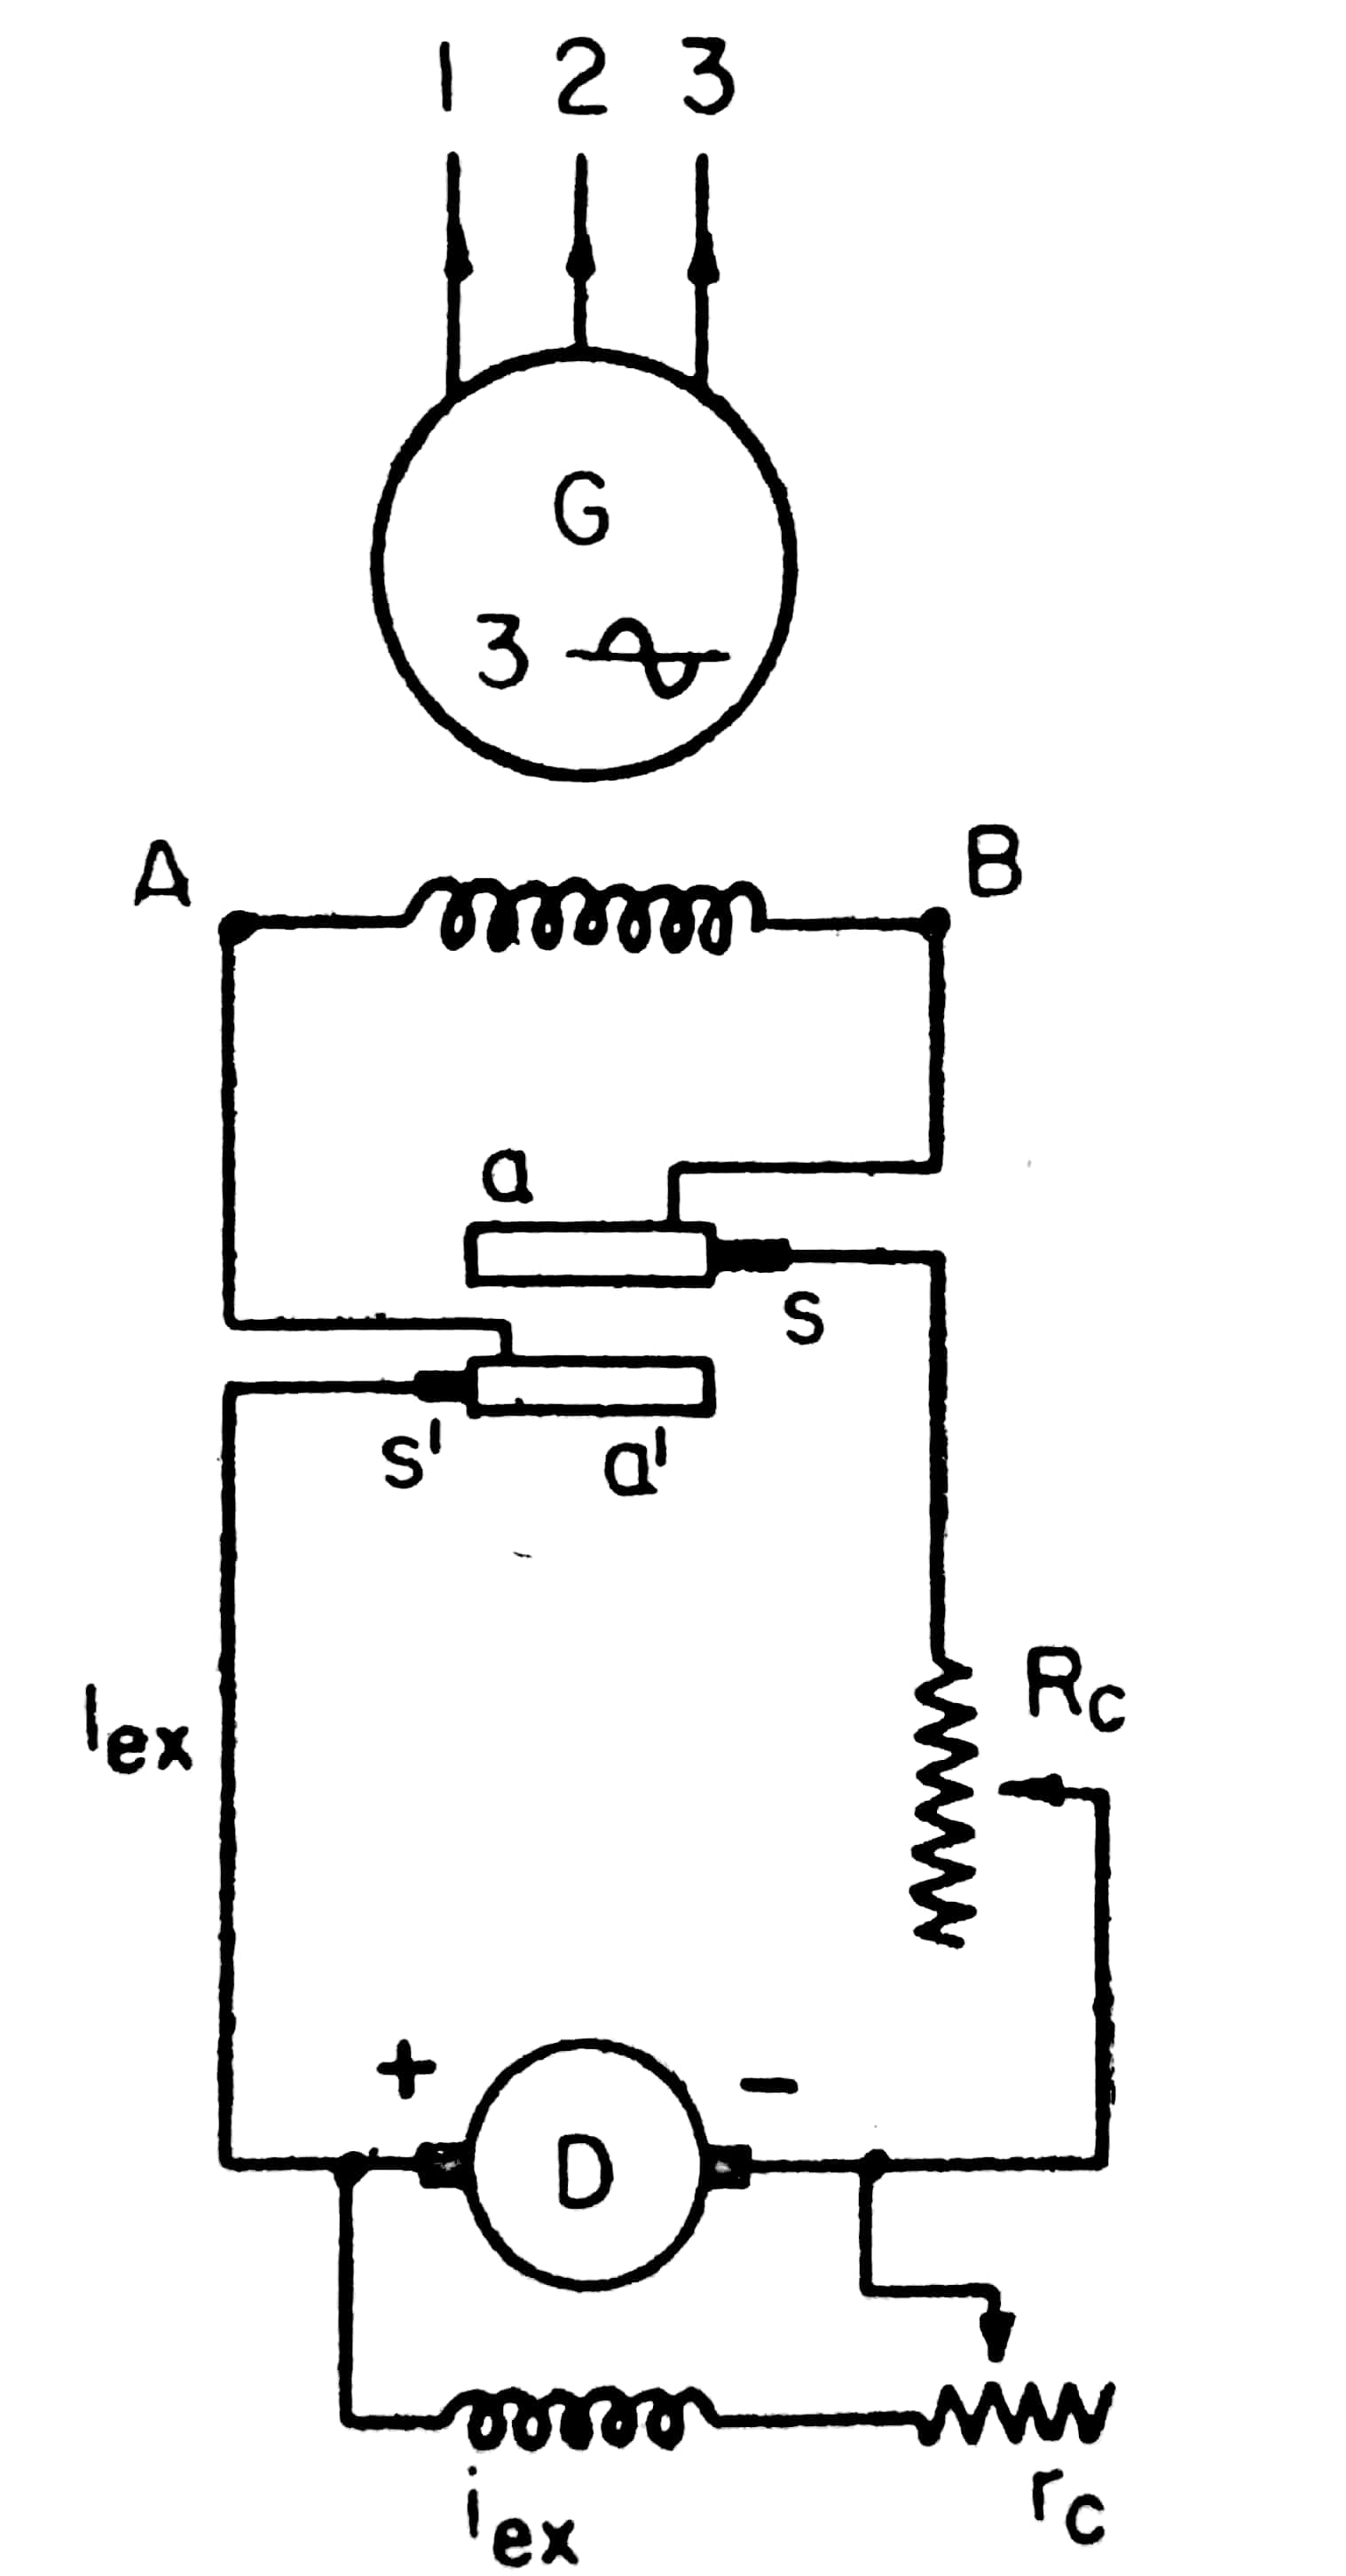
\includegraphics[scale=0.2]{imagens/19.png}
\caption{Esquema elétrico.}
\end{figure}

Os terminais 1,2 e 3 são fixos no alternador. A-B são os terminais de enrolamento indutor rotativo, ligado aos anéis $a$ e $a'$, fixos sobre o eixo: Sobre os anéis apoiam-se as escovas $S$ e $S'$, com as quais estão ligadas as conexões provenientes das escovas (+) e (-) do dínamo excitador. Sobre uma dessas conexões é inserido o reostato $R_c$. A regulação da corrente de excitação do alternador pode ser feita de duas maneiras, ou seja, por meio do reostato de campo do alternador $R_c$, ou regulando-se o reostato de campo $r_c$ do dínamo excitador.

